\section{Implementation steps}


\section{Results}

The results varied quite a bit, which I guess is somewhat expected due to the
iterative nature of RANSAC\@. Still, there was considerable variance between
runs.

The parameter with the biggest influence on results was the distance threshold.
Smaller thresholds usually come up with the best results, but they were also
far more unstable. Larger thresholds were more stable, but never gave any
really good results.

Choosing the threshold also seems to be dependent on the quality of the feature
extractor; Features from a bad extractor have more outliers, and thus it's
preferable to have a smaller threshold. And vice versa with a good extractor.
Unfortunately, it also seems that the threshold needed to be selected according
to the picture pair, which is quite undesireable behaviour.

Table~\ref{tab:homographies} contains the resulting homographies for both image
pairs.

\begin{table}[H]
  \caption{The best homographies for both image pairs, obtained by the RANSAC
  algorithm}\label{tab:homographies}
  \begin{minipage}{.5\linewidth}
    \caption{H1 image pair best homography}
    \centering
    \begin{tabular}{rrr}
      \toprule
       5.22E-01 & -1.49E-01 & 6.06E+01 \\
      -5.49E-02 &  4.98E-01 & 1.07E+02 \\
      -9.04E-05 & -1.65E-04 & 7.53E-01 \\
      \bottomrule
    \end{tabular}
  \end{minipage}
  \begin{minipage}{.5\linewidth}
    \centering
    \caption{H2 image pair best homography}
    \begin{tabular}{rrr}
      \toprule
      3.28E-01 & -4.11E-03 & 2.39E+02 \\
      2.63E-02 &  2.65E-01 & 1.11E+02 \\
      1.11E-04 & -3.94E-06 & 4.52E-01 \\
      \bottomrule
    \end{tabular}
  \end{minipage} 
\end{table}

\subsection{Visualization}

\subsubsection{Image pair H1 visualization}

\begin{figure}[H]
  \centering
  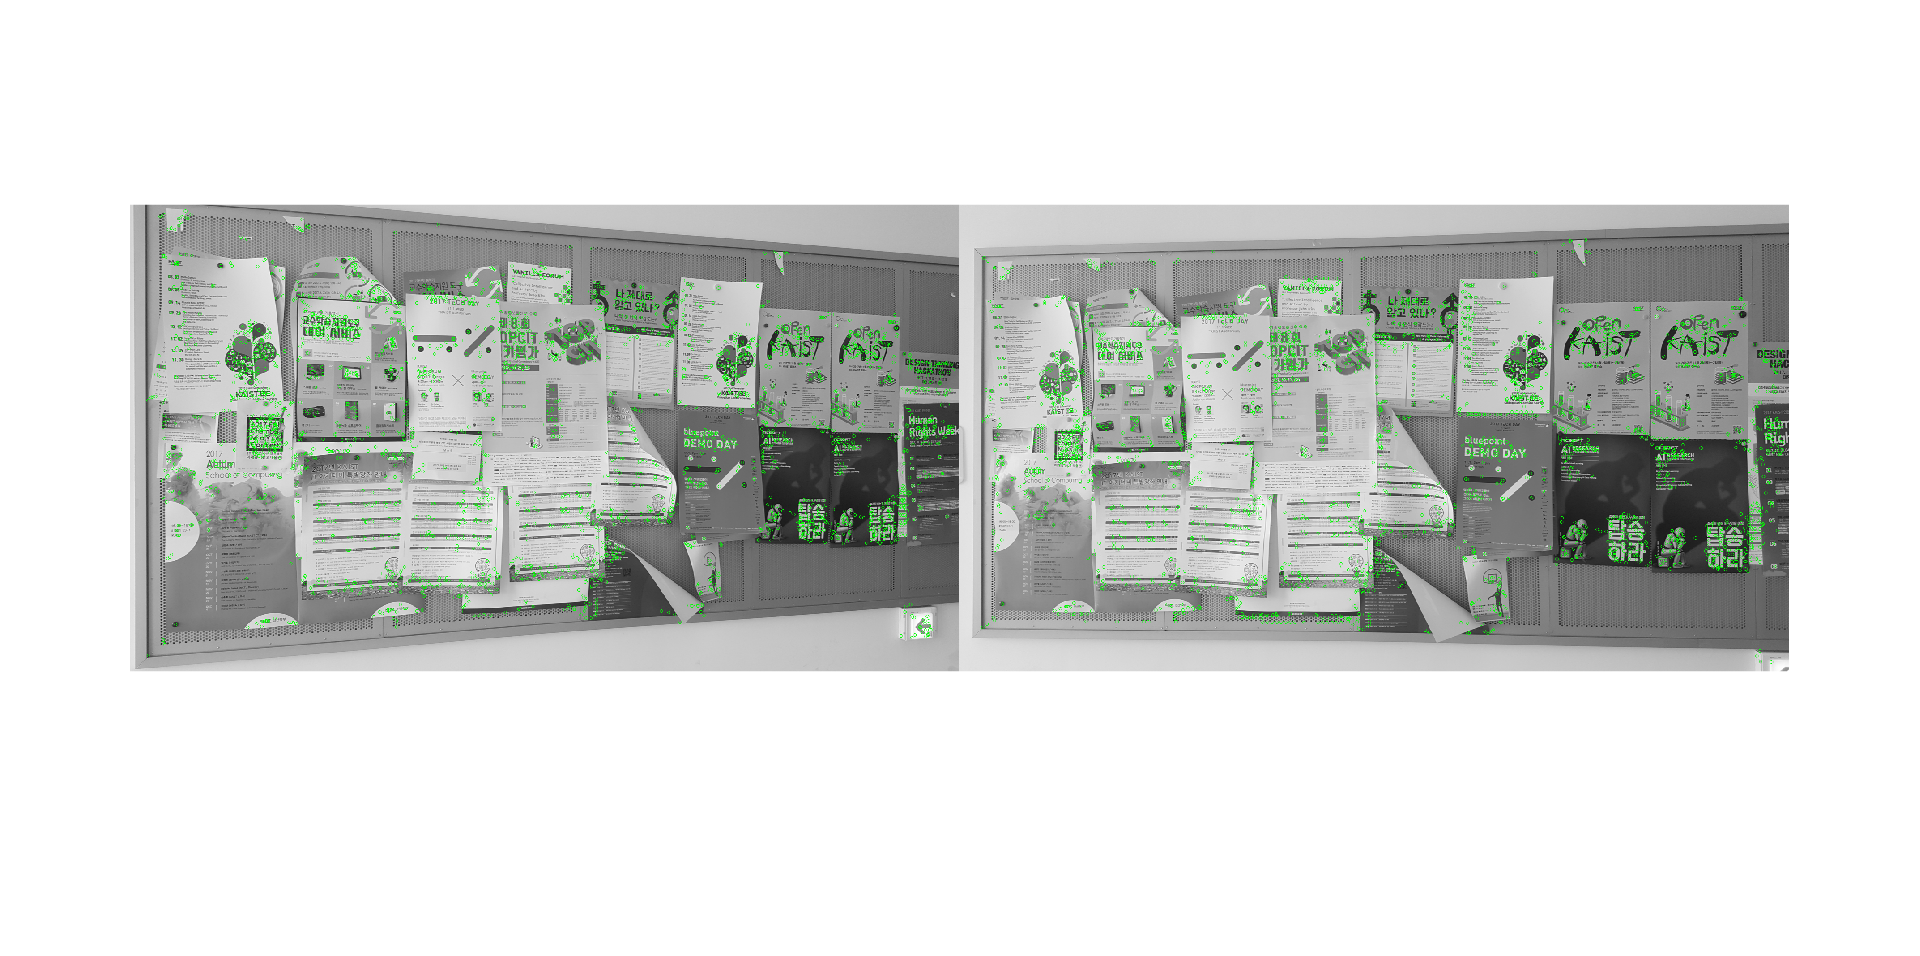
\includegraphics[width=1\linewidth]{H1_interest_points}
  \caption{Found interest points}
\end{figure}

\begin{figure}[H]
  \centering
  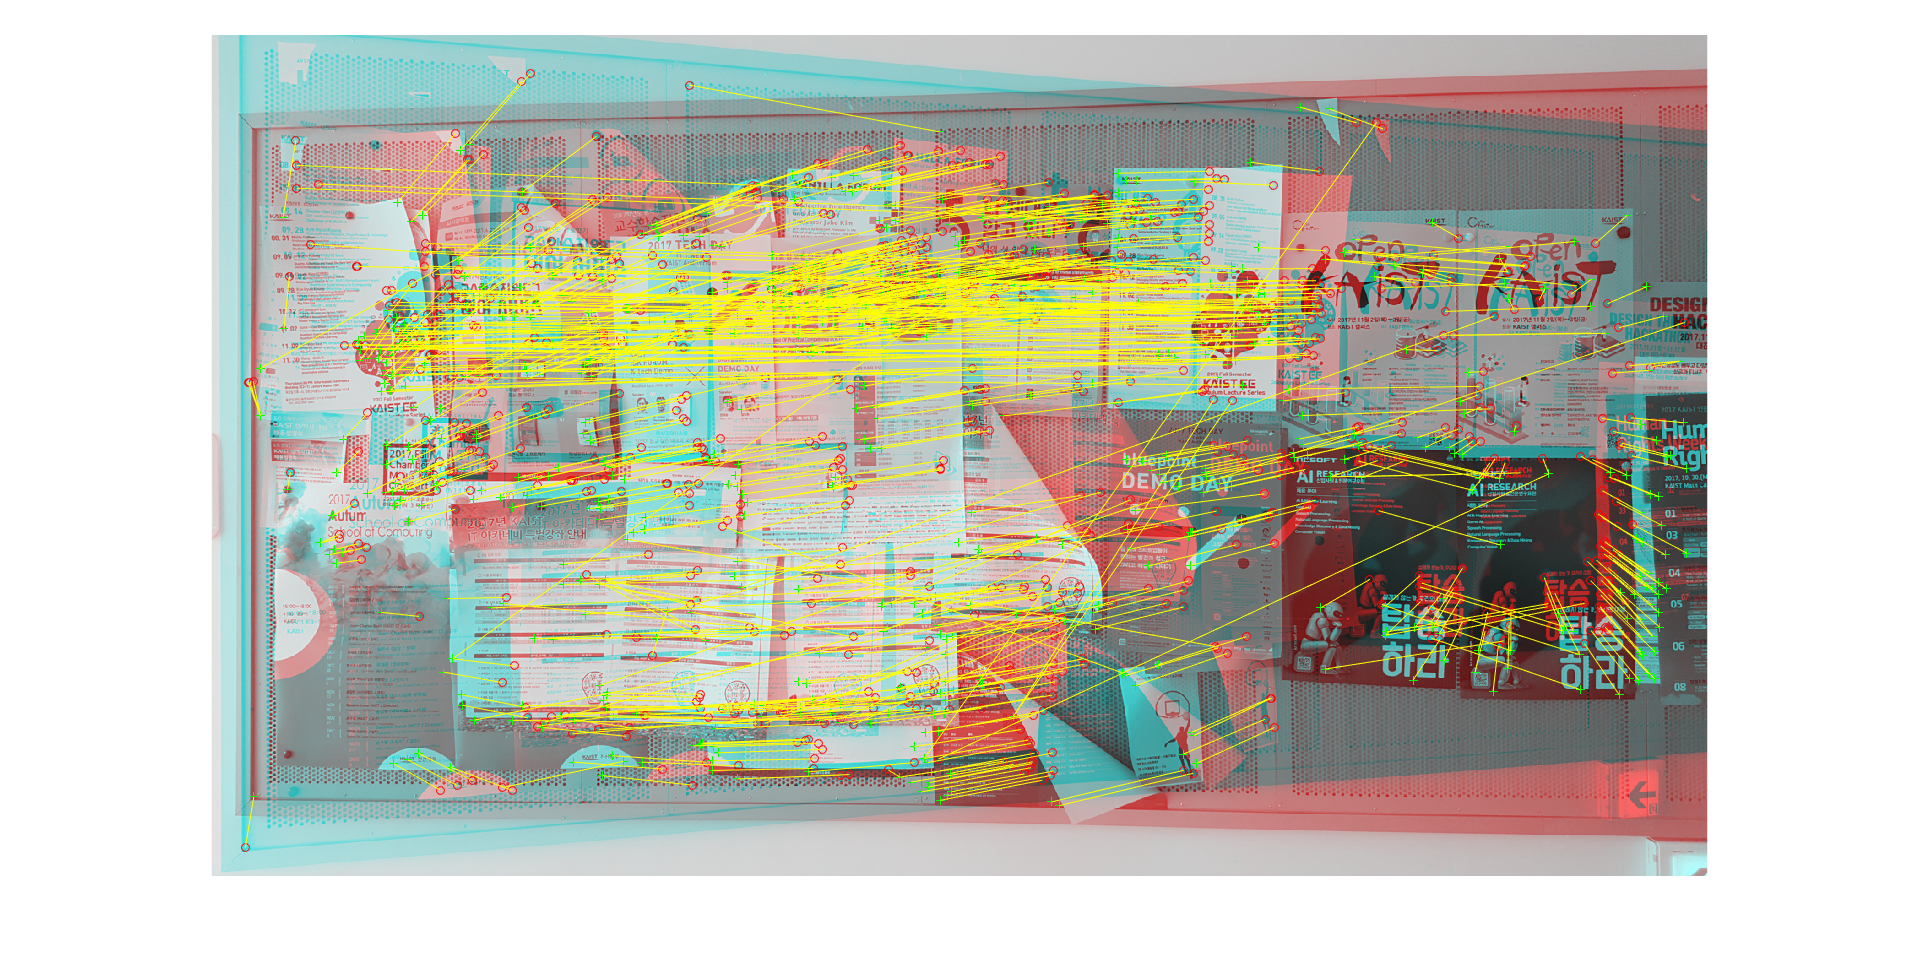
\includegraphics[width=1\linewidth]{H1_correspondences}
  \caption{Matches between interest points}
\end{figure}

\begin{figure}[H]
  \centering
  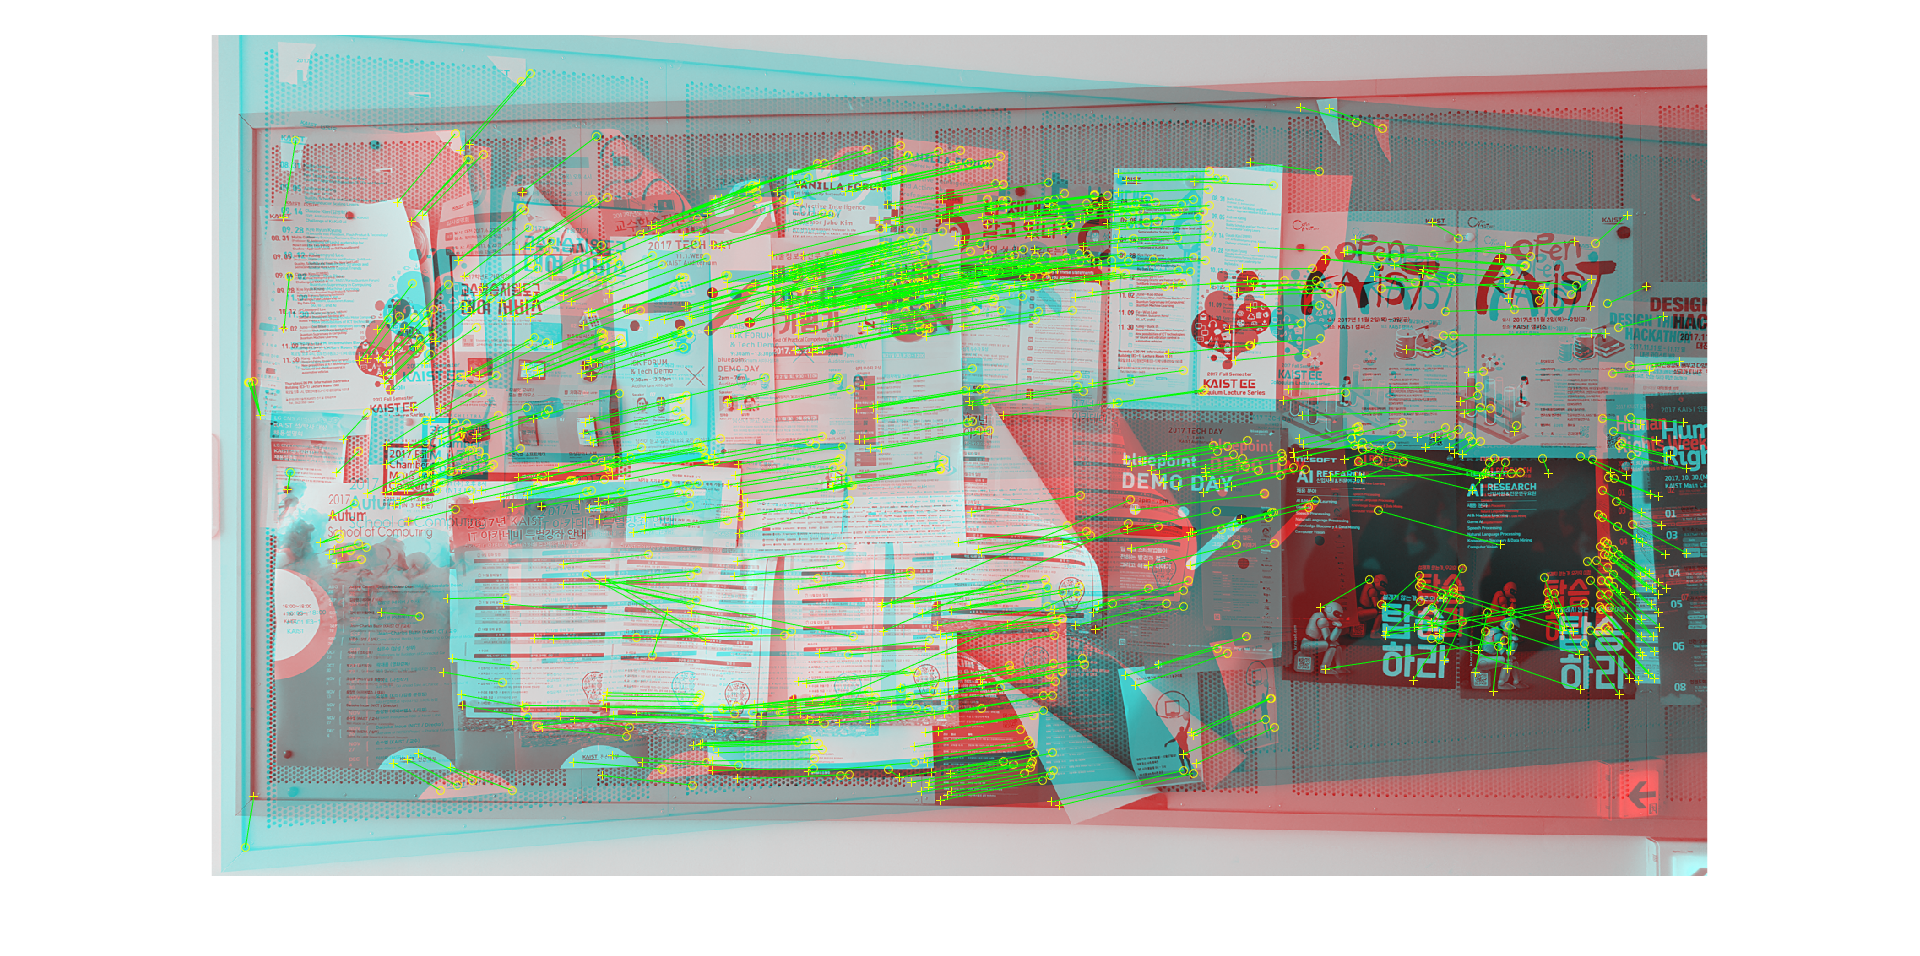
\includegraphics[width=1\linewidth]{H1_inliers}
  \caption{Inliers from the best fitting homography obtained by RANSAC}
\end{figure}

\begin{figure}[H]
  \centering
  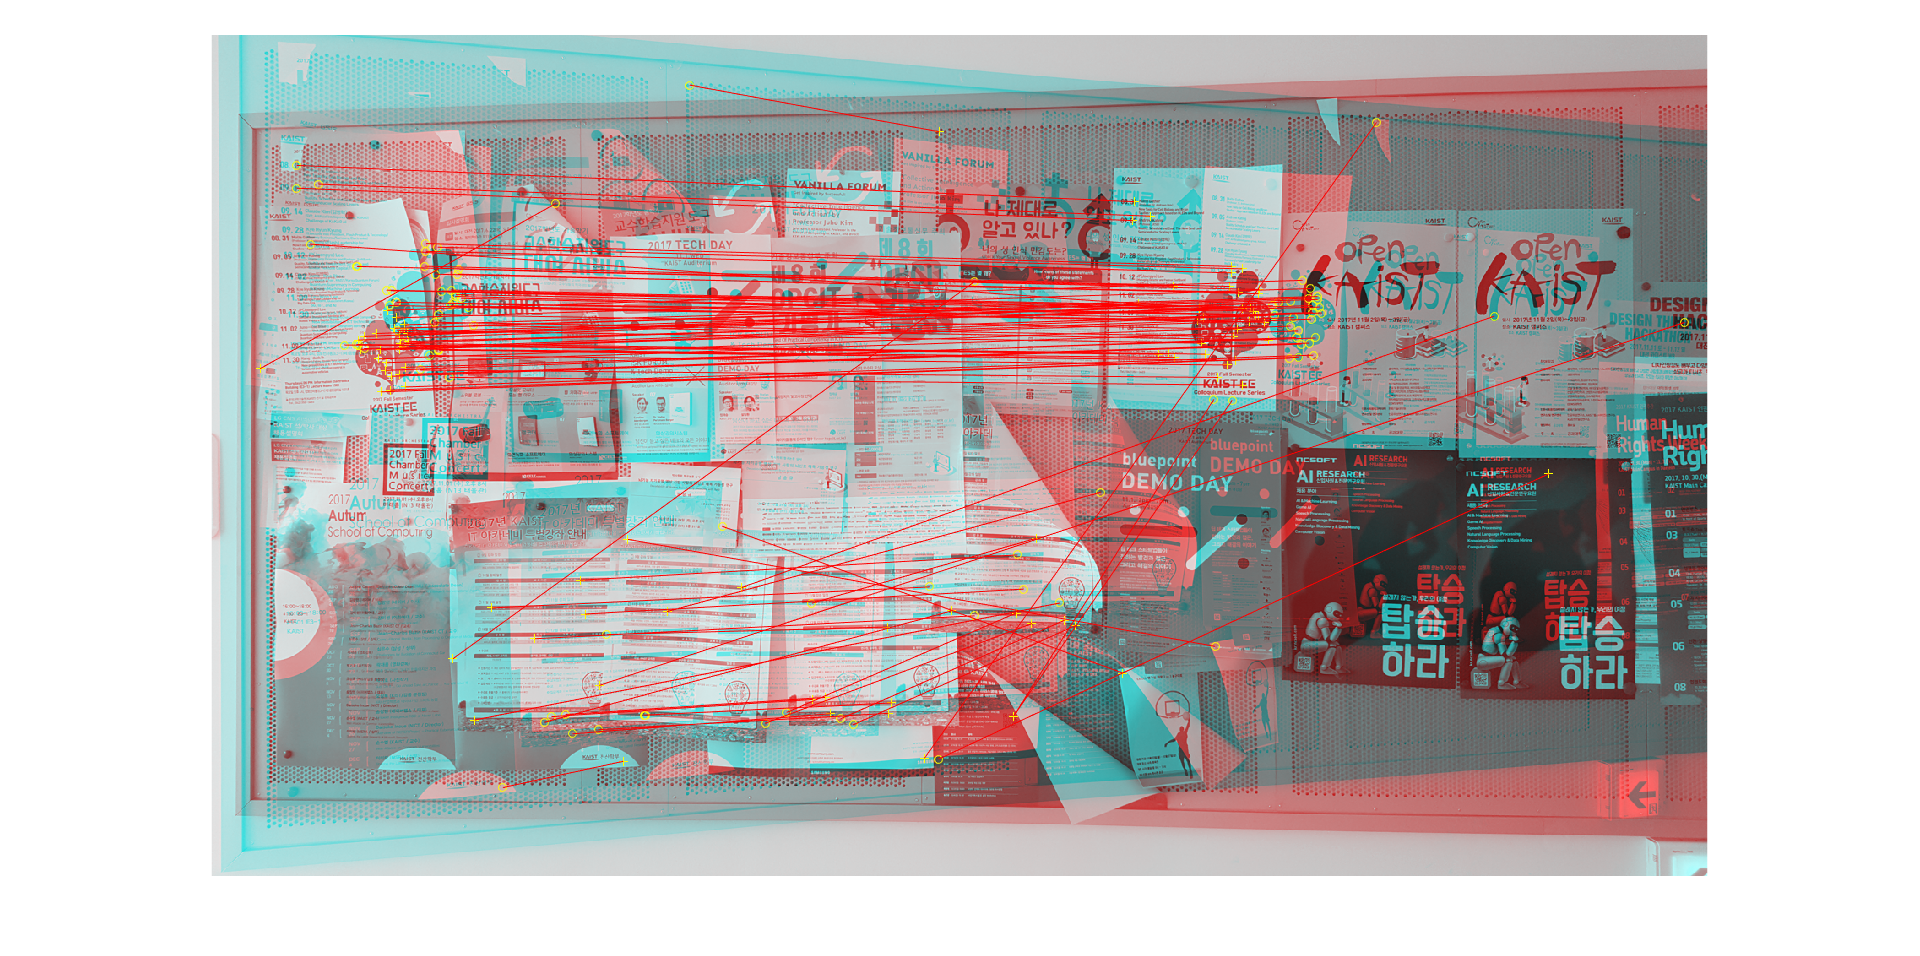
\includegraphics[width=1\linewidth]{H1_outliers}
  \caption{Outliers from the best fitting homography obtained by RANSAC}
\end{figure}

\begin{figure}[H]
  \centering
  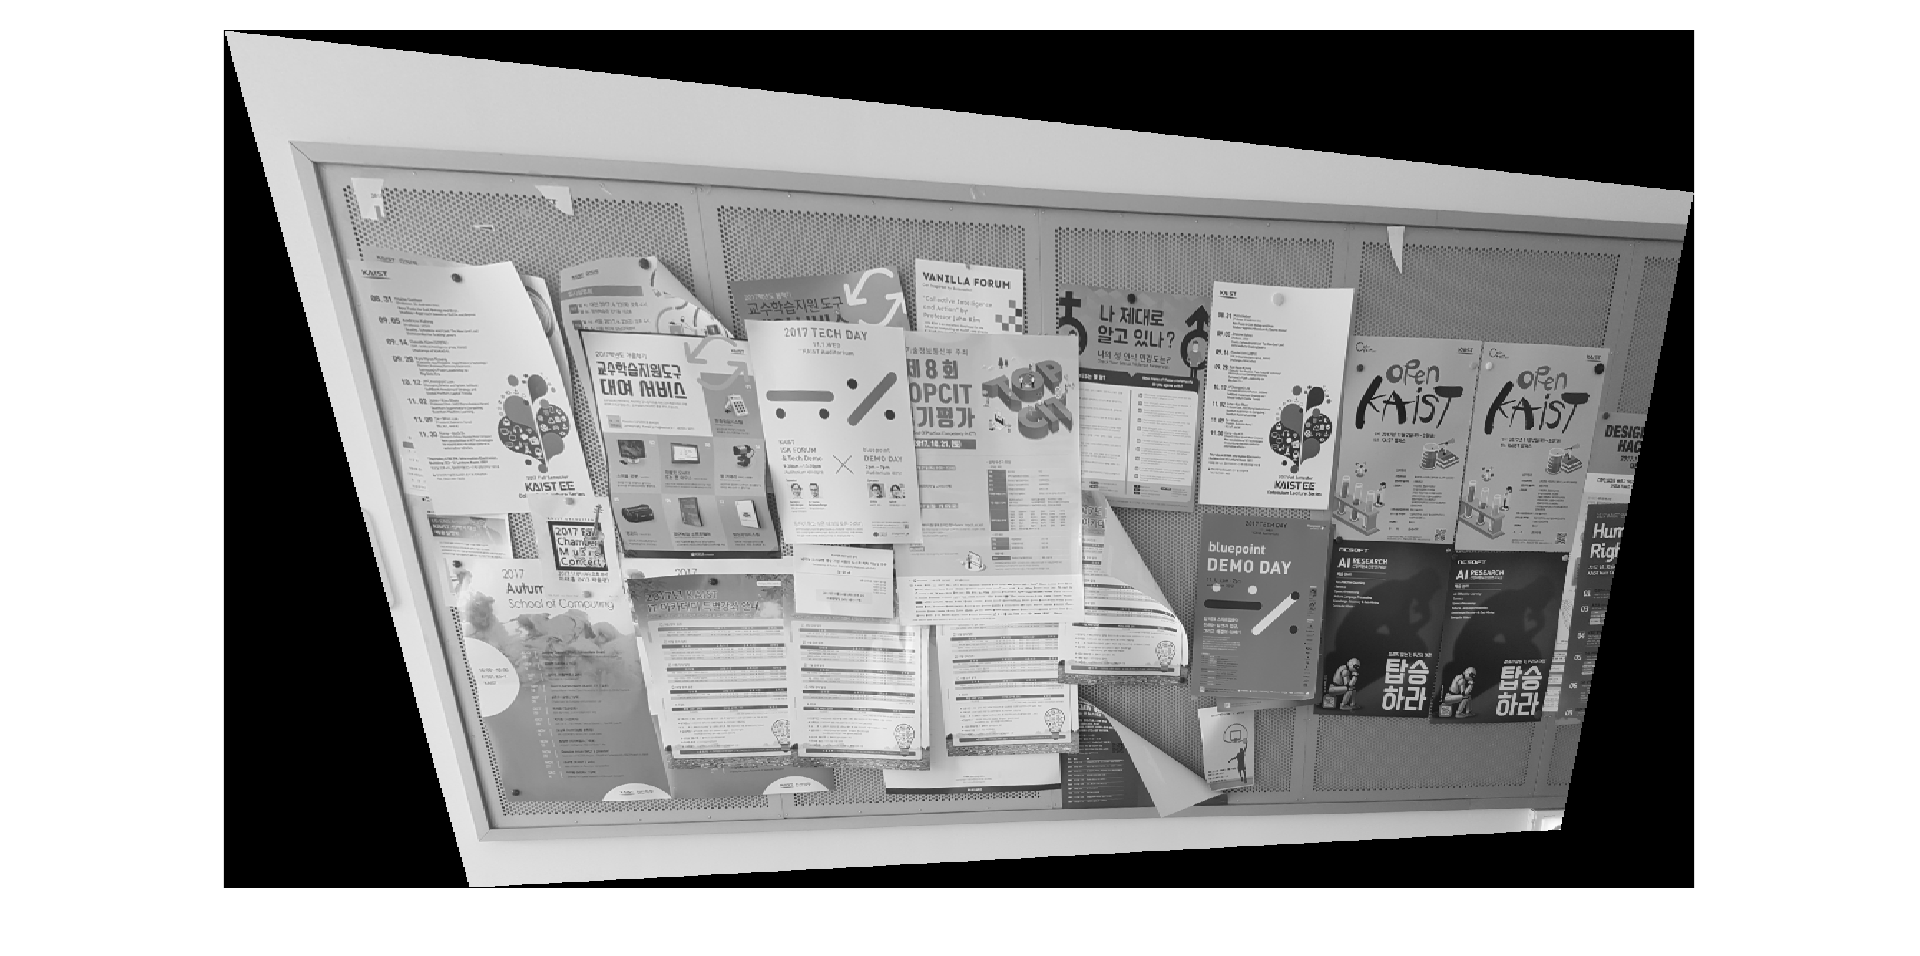
\includegraphics[width=1\linewidth]{H1_best_H}
  \caption{The second image transformed by the homography obtained with RANSAC}
\end{figure}

\begin{figure}[H]
  \centering
  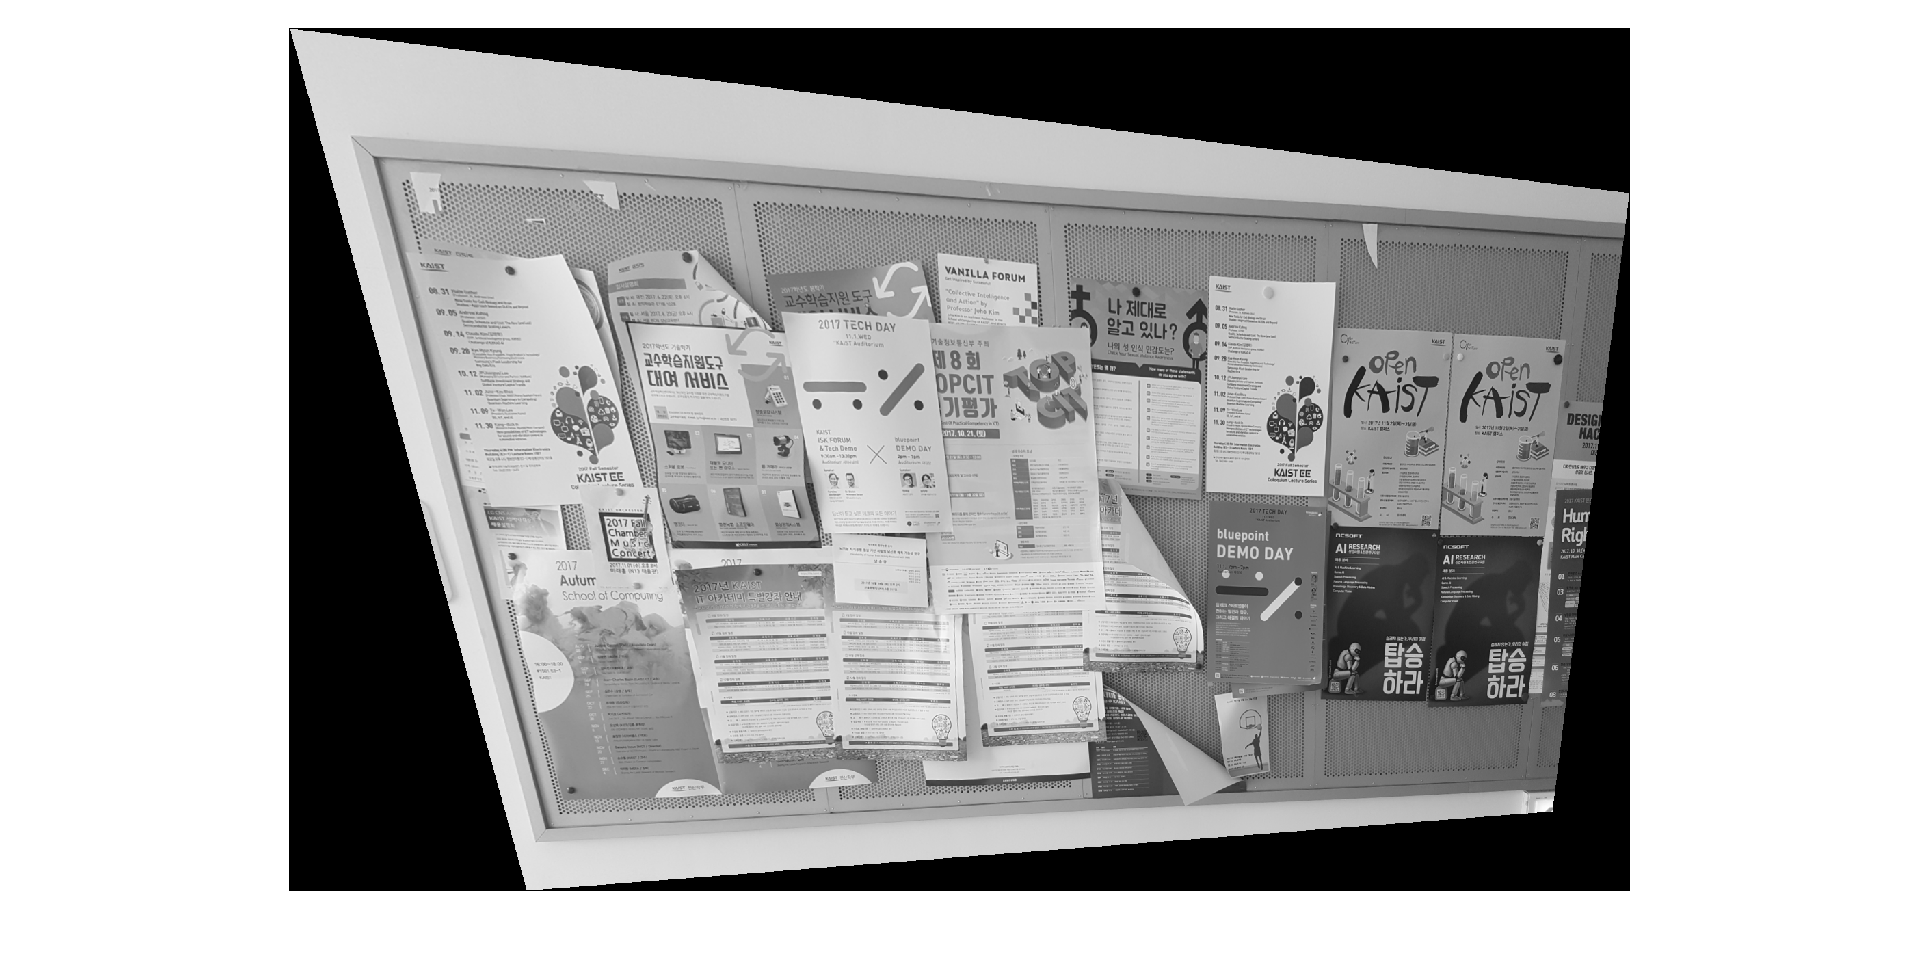
\includegraphics[width=1\linewidth]{H1_optimal_H}
  \caption{The second image transformed by the homography obtained from the
  inliers using the Levenberg-Marquadt fitting algorithm}
\end{figure}


\subsubsection{Image pair H2 visualization}

\begin{figure}[H]
  \centering
  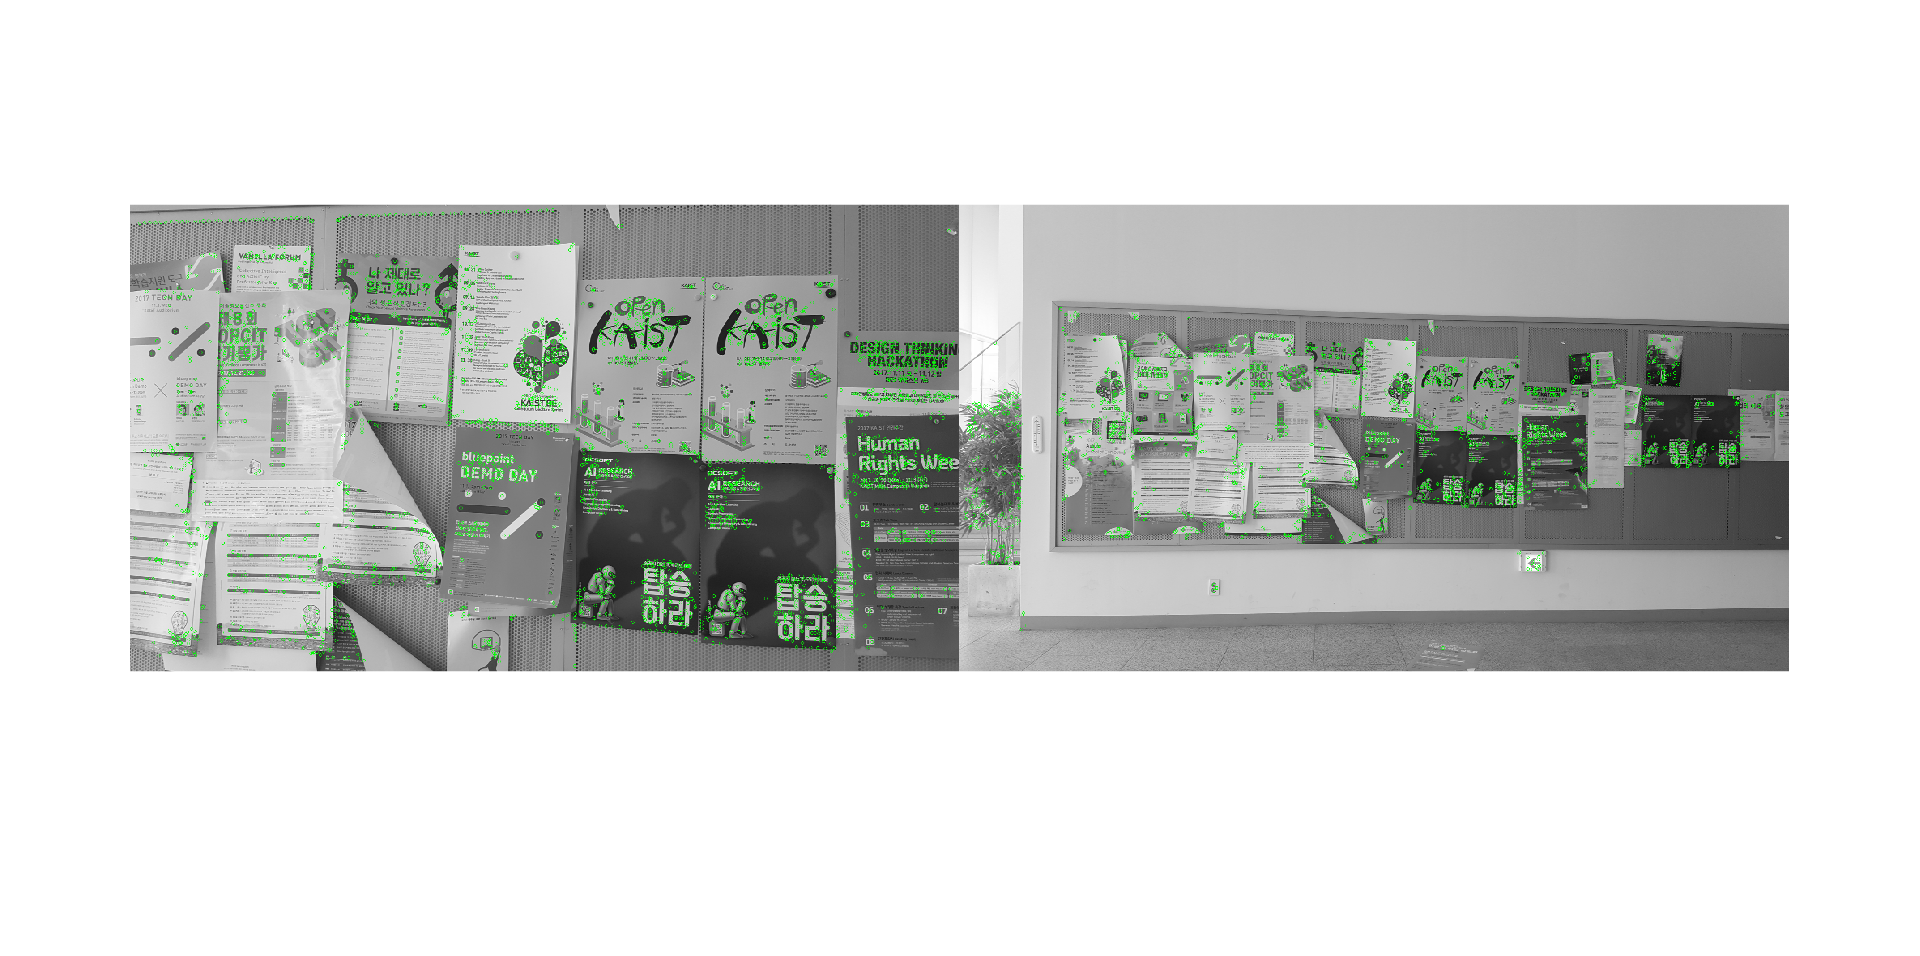
\includegraphics[width=1\linewidth]{H2_interest_points}
  \caption{Found interest points}
\end{figure}

\begin{figure}[H]
  \centering
  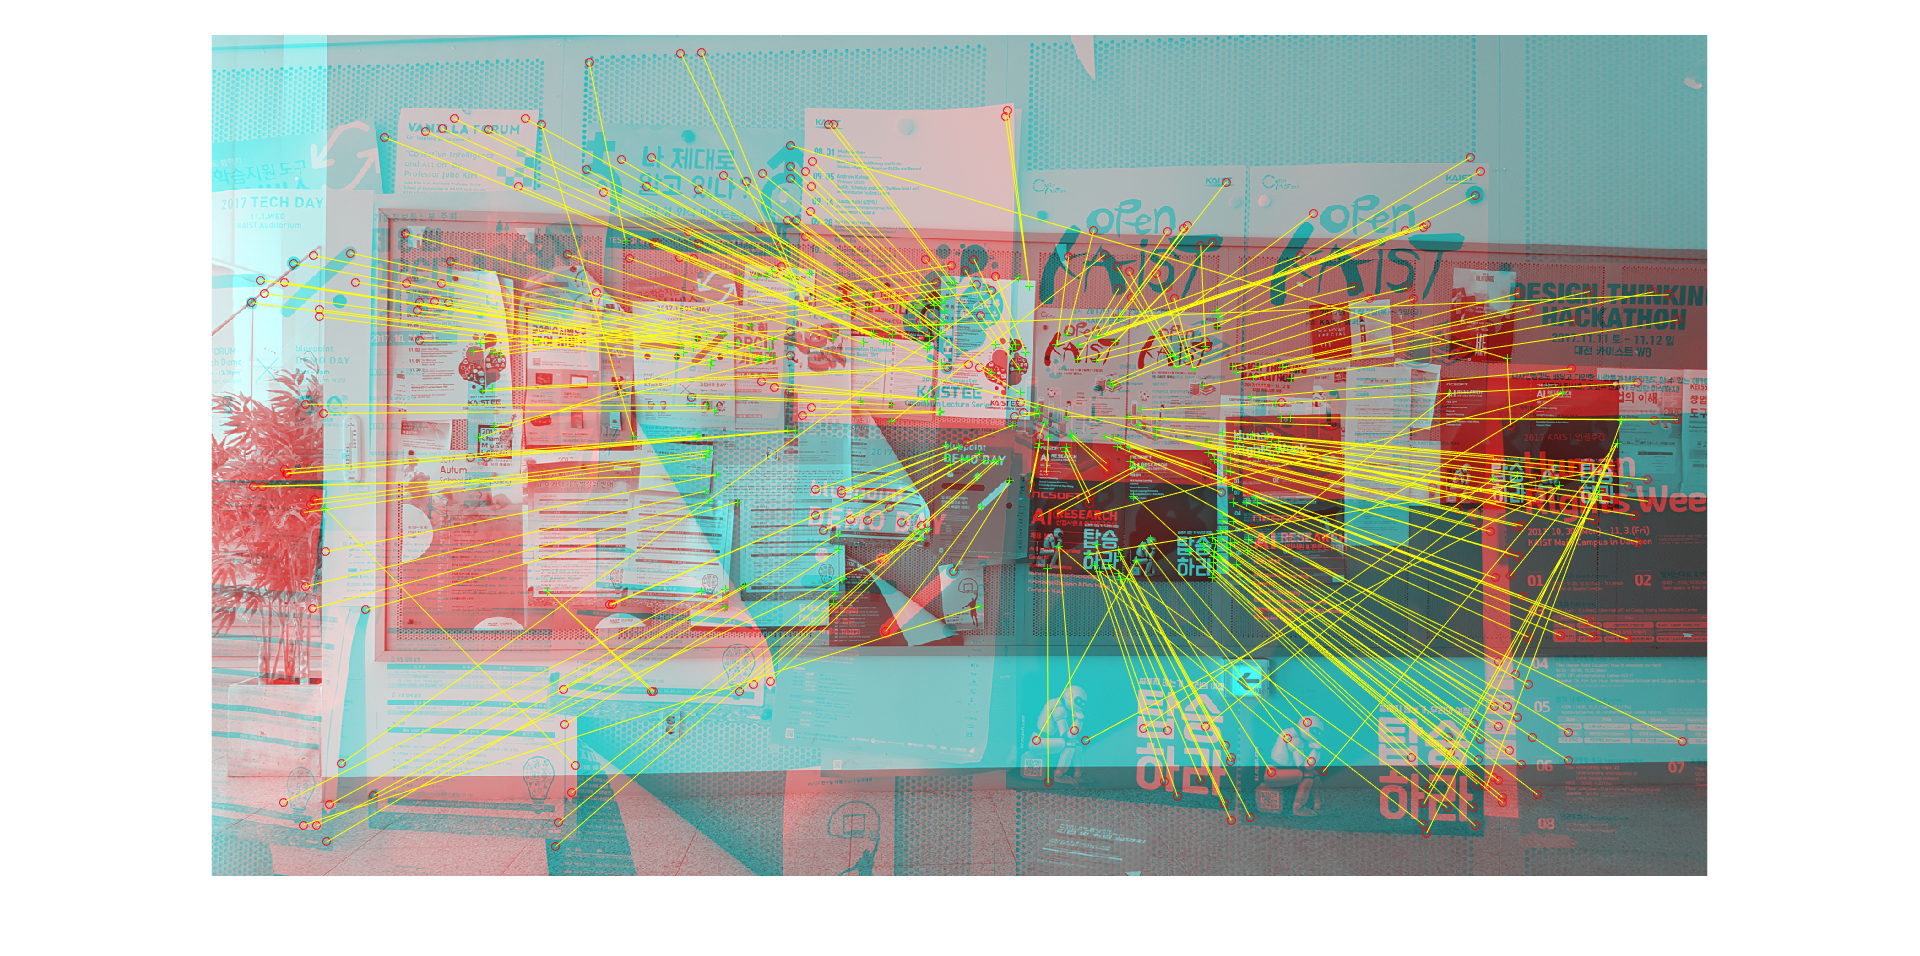
\includegraphics[width=1\linewidth]{H2_correspondences}
  \caption{Matches between interest points}
\end{figure}

\begin{figure}[H]
  \centering
  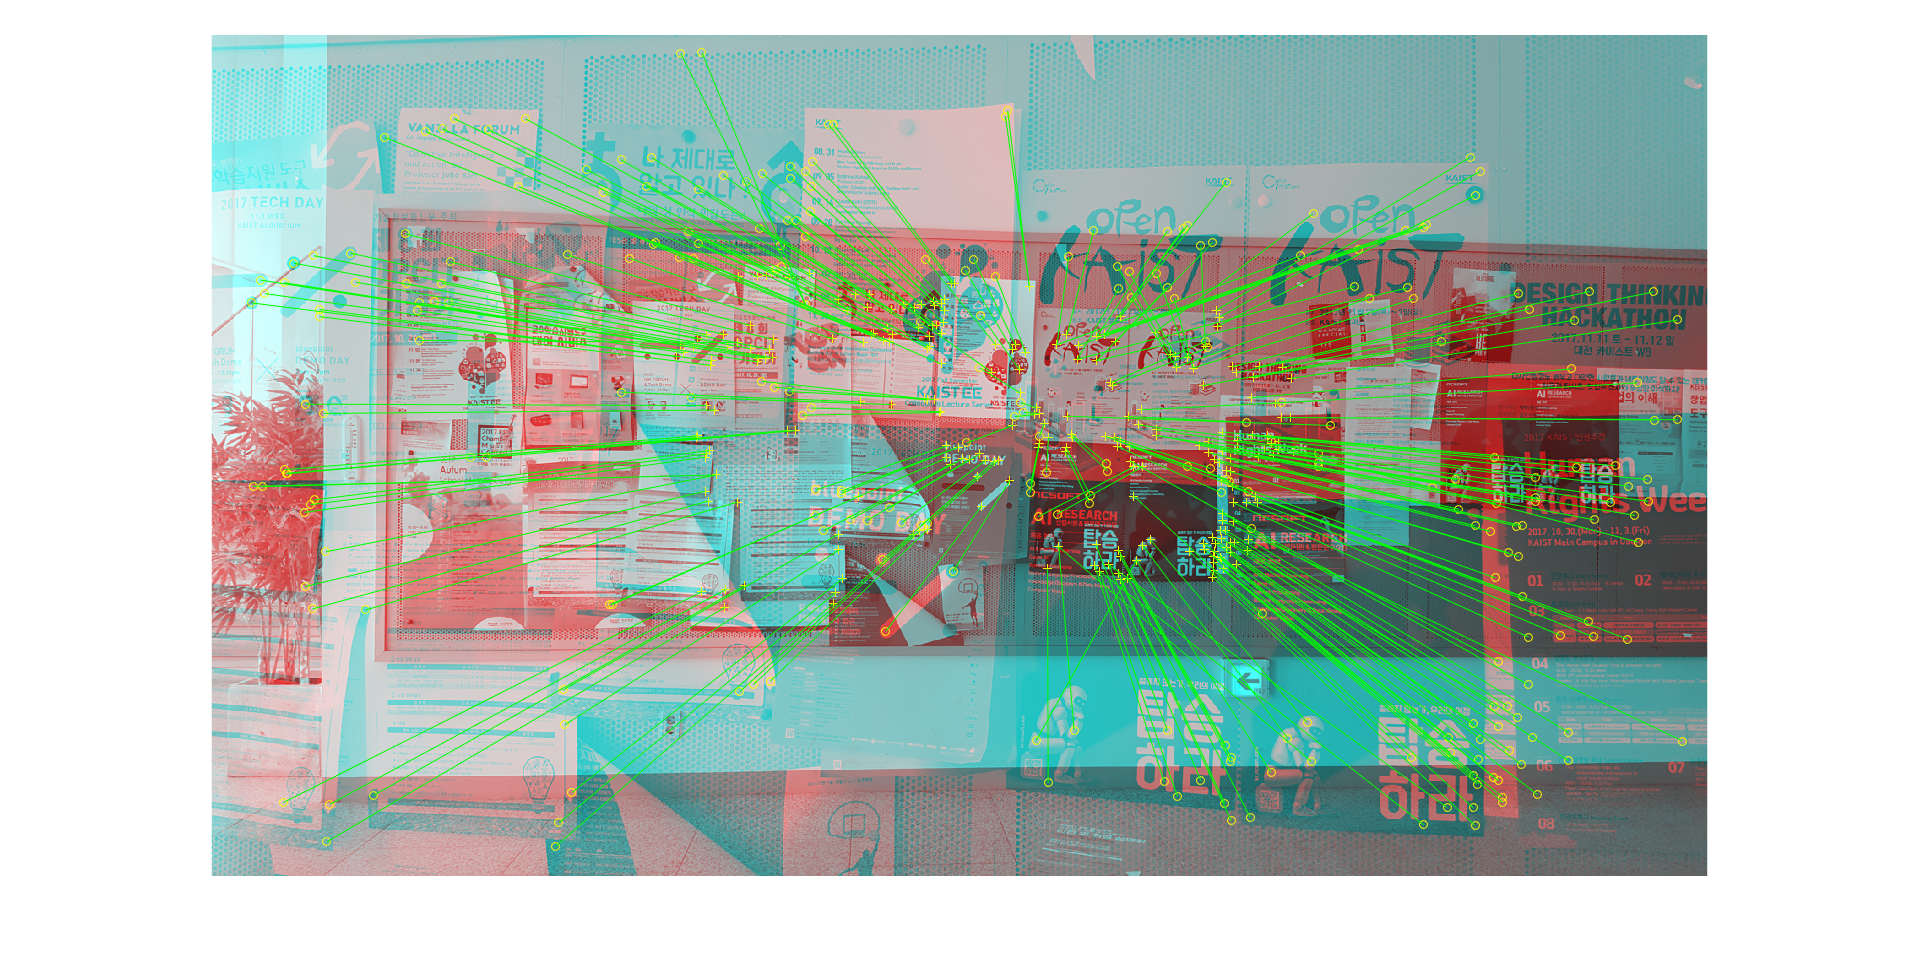
\includegraphics[width=1\linewidth]{H2_inliers}
  \caption{Inliers from the best fitting homography obtained by RANSAC}
\end{figure}

\begin{figure}[H]
  \centering
  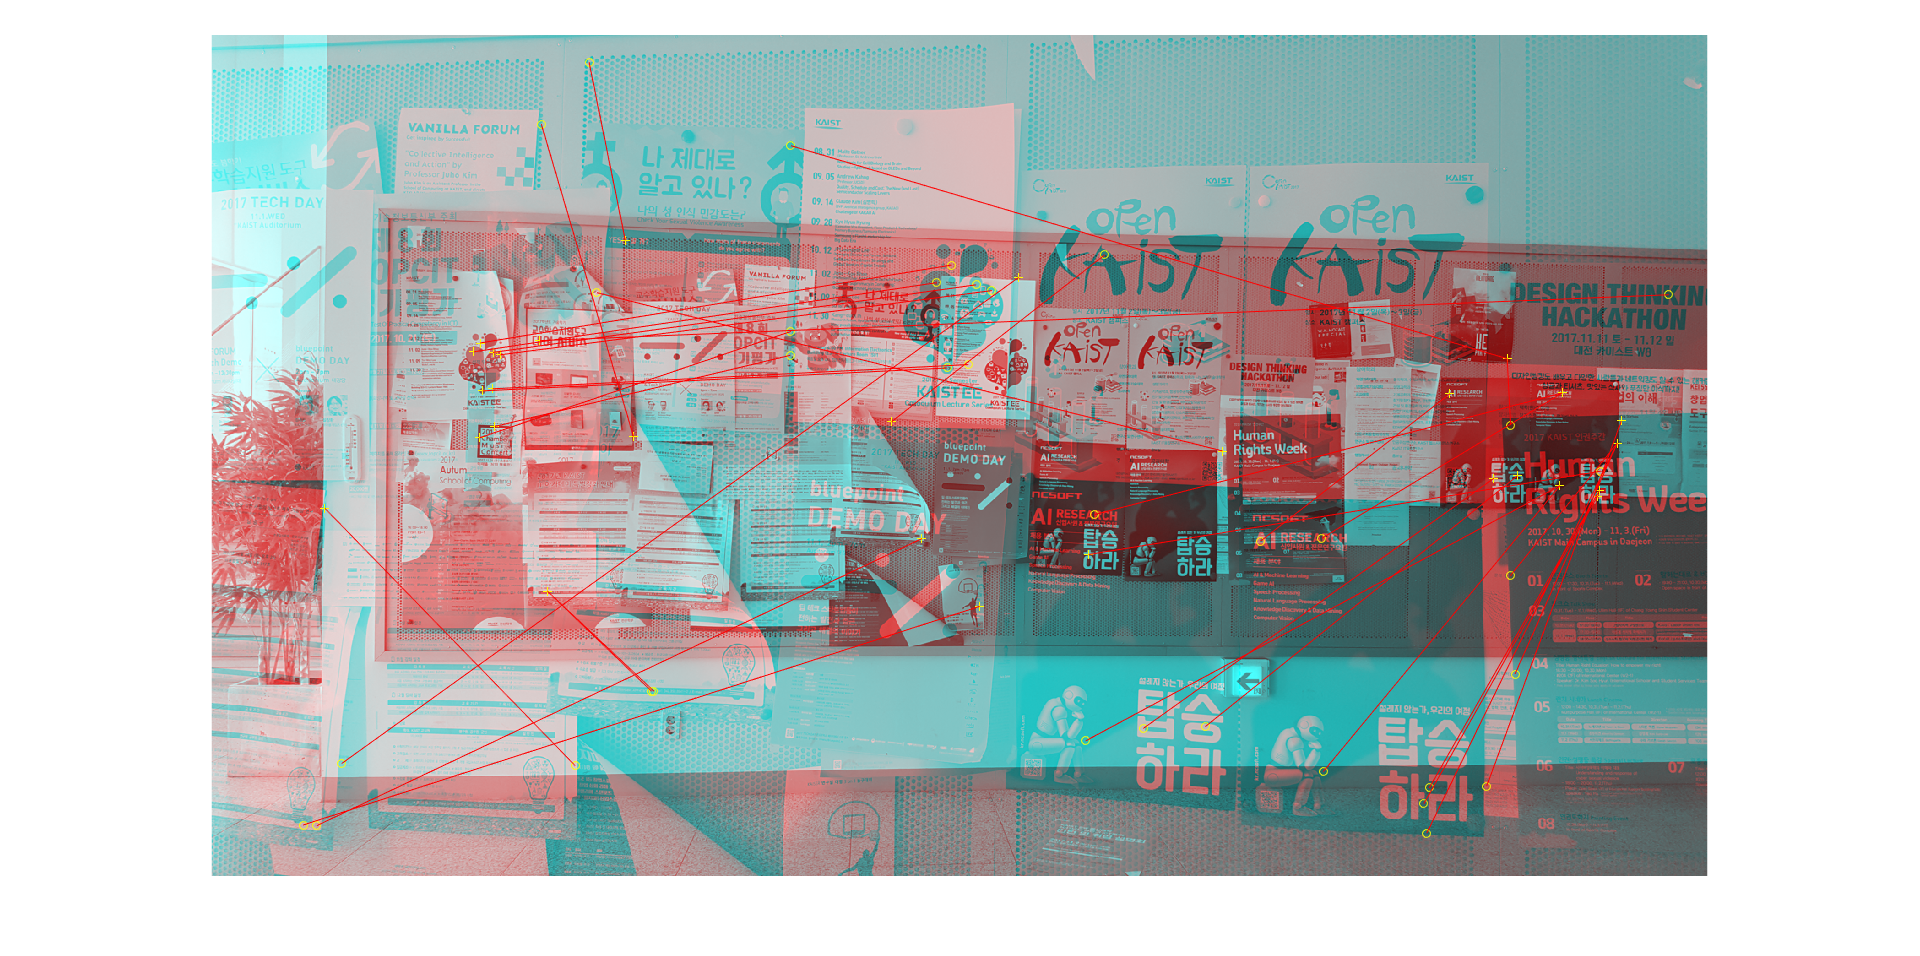
\includegraphics[width=1\linewidth]{H2_outliers}
  \caption{Outliers from the best fitting homography obtained by RANSAC}
\end{figure}

\begin{figure}[H]
  \centering
  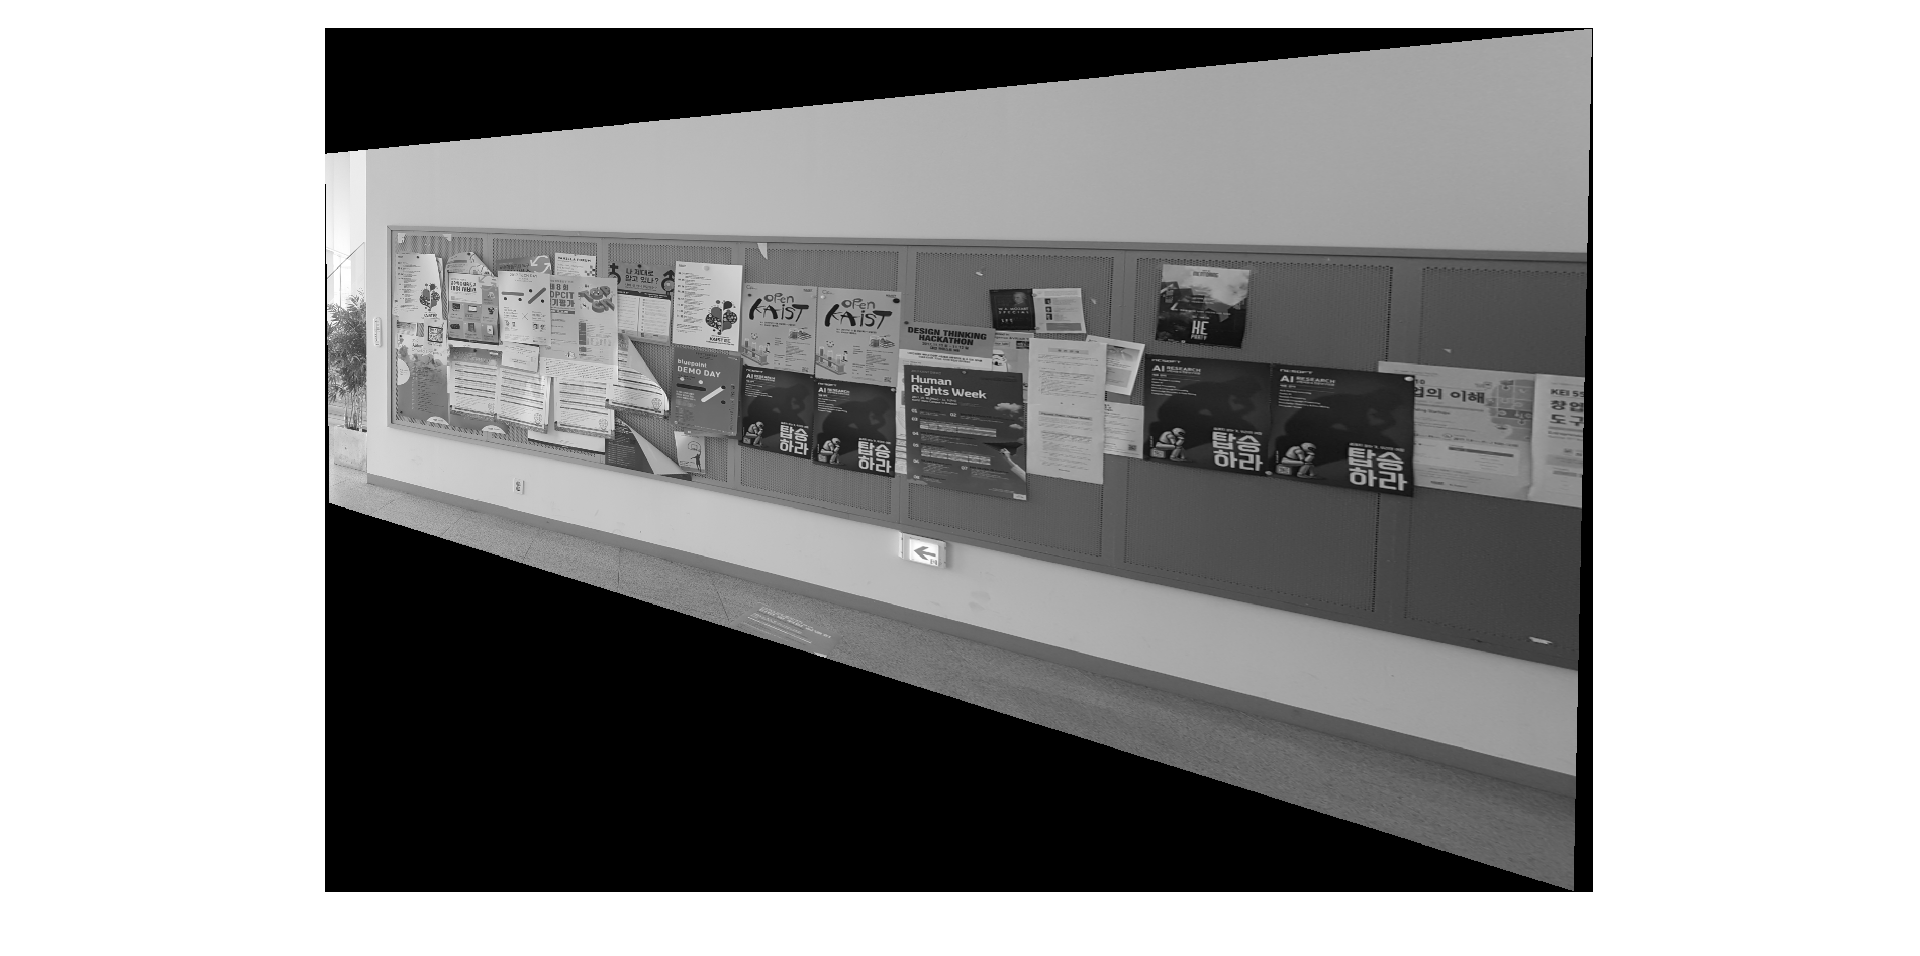
\includegraphics[width=1\linewidth]{H2_best_H}
  \caption{The second image transformed by the homography obtained with RANSAC}
\end{figure}

\begin{figure}[H]
  \centering
  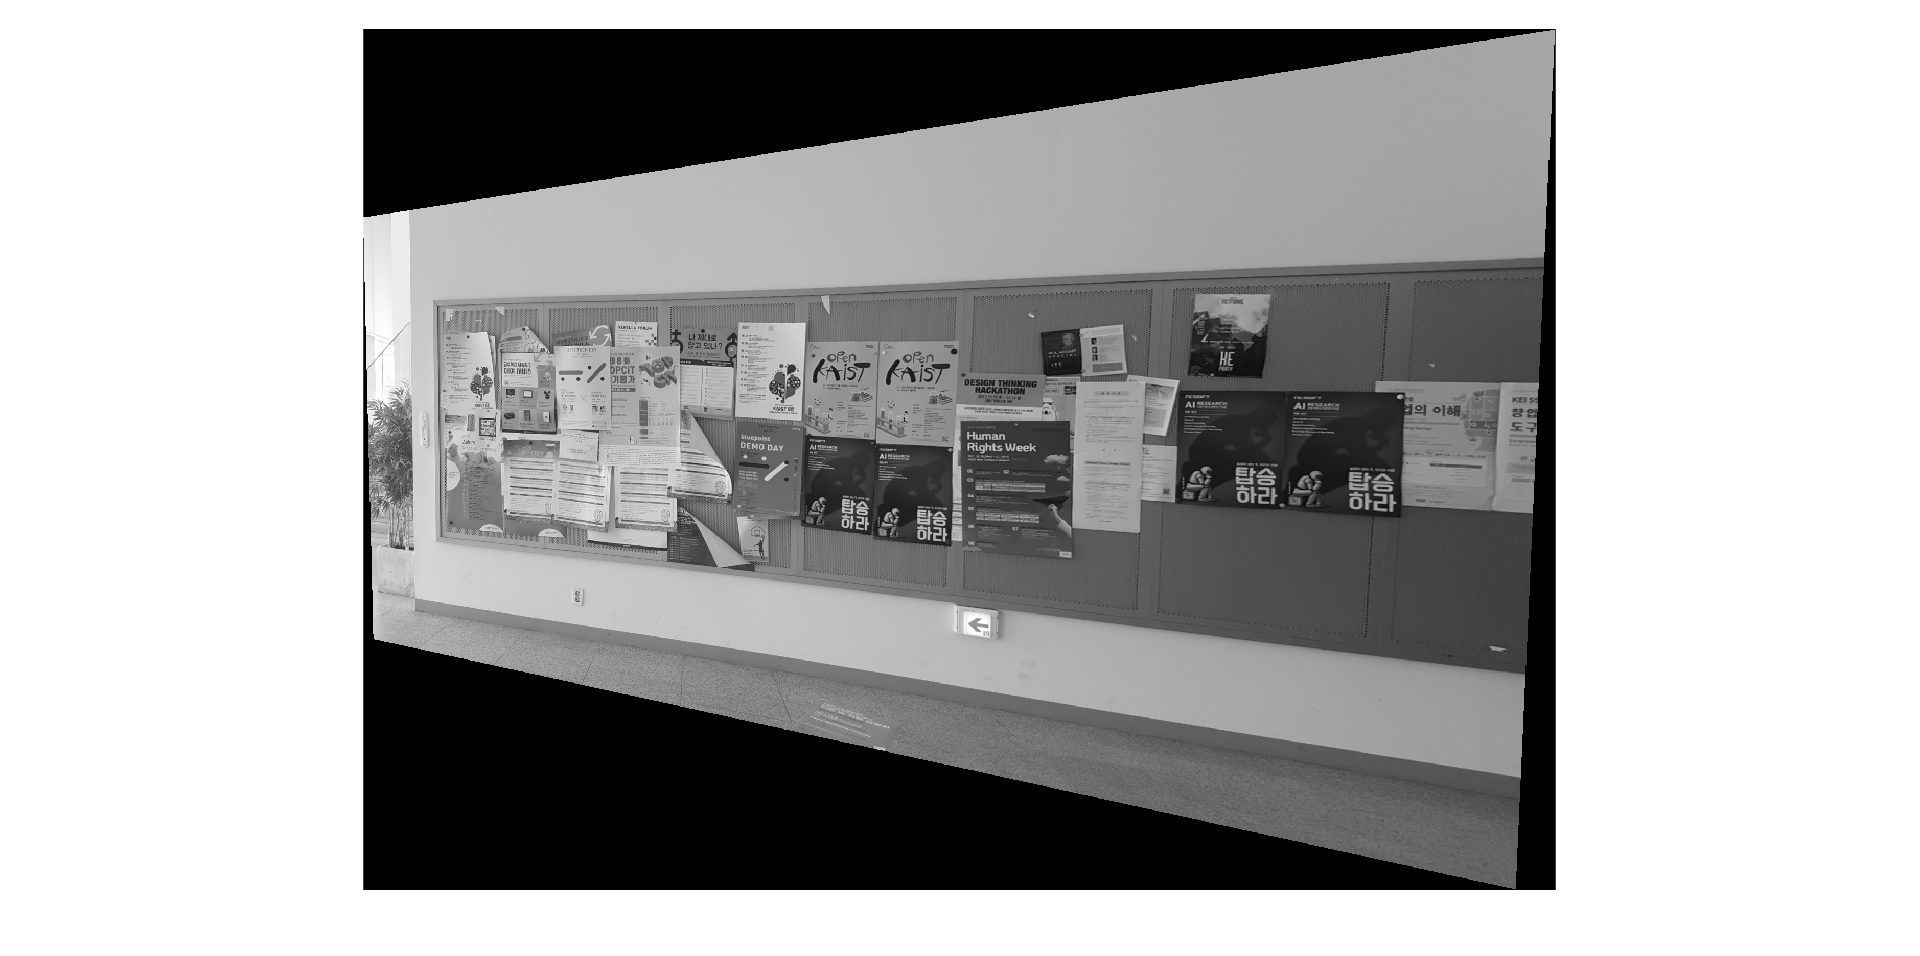
\includegraphics[width=1\linewidth]{H2_optimal_H}
  \caption{The second image transformed by the homography obtained from the
  inliers using the Levenberg-Marquadt fitting algorithm}
\end{figure}
